\documentclass[
	% -- opções da classe memoir --
	12pt,				% tamanho da fonte
	openright,			% capítulos começam em pág ímpar (insere página vazia caso preciso)
	oneside,			% para impressão em verso e anverso. Oposto a oneside
	a4paper,			% tamanho do papel. 
	% -- opções do pacote babel --
	% idioma adicional para hifenização
	brazil,				% o último idioma é o principal do documento
	]{abntex2}


\usepackage{cmap}				% Mapear caracteres especiais no PDF
\usepackage{lmodern}			% Usa a fonte Latin Modern			
\usepackage[T1]{fontenc}		% Selecao de codigos de fonte.
\usepackage[utf8]{inputenc}		% Codificacao do documento (conversão automática dos acentos)
\usepackage{lastpage}			% Usado pela Ficha catalográfica
\usepackage{indentfirst}		% Indenta o primeiro parágrafo de cada seção.
\usepackage{color}				% Controle das cores
\usepackage{graphicx}			% Inclusão de gráficos
\usepackage{amsmath}
\usepackage{mathtools}

\usepackage[brazilian,hyperpageref]{backref}	 % Paginas com as citações na bibl
\usepackage[alf]{abntex2cite}	% Citações padrão ABNT

% Incluir código fonte
%\usepackage{minted}

% Use wide margins, but not quite so wide as fullpage.sty
\marginparwidth 0.5in 
\oddsidemargin 0.25in 
\evensidemargin 0.25in 
\marginparsep 0.25in
\topmargin 0.25in 
\textwidth 6in \textheight 8 in
% That's about enough definitions

% multirow allows you to combine rows in columns
\usepackage{multirow}
% tabularx allows manual tweaking of column width
\usepackage{tabularx}
% longtable does better format for tables that span pages
\usepackage{longtable}


\titulo{Título do trabalho}
\author{Discentes:\\\hspace{2cm}Sicrano\\\hspace{2cm}Beltrano\\\hspace{2cm}Fulano\\}
\orientador{Kennedy Reurison Lopes}
\instituicao{%
  Universidade Federal do Rio Grande do Norte
  \par
  Centro de Tecnologia
  \par
  Departamento de Computação e Automação
  \par
  Engenharia de Computação}

\local{Natal}
\date{08 de março de 2019}



% ---
% Configurações de aparência do PDF final

% informações do PDF
\makeatletter
\hypersetup{
     	%pagebackref=true,
		pdftitle={\@title}, 
		pdfauthor={\@author},
    	pdfsubject={\imprimirpreambulo},
	    pdfcreator={LaTeX with abnTeX2},
		pdfkeywords={abnt}{latex}{abntex}{abntex2}{trabalho acadêmico}, 
		colorlinks=true,       		% false: boxed links; true: colored links
    	linkcolor=black,          	% color of internal links
    	citecolor=black,        		% color of links to bibliography
    	filecolor=black,      		% color of file links
		urlcolor=black,
		bookmarksdepth=4
}
\makeatother
% --- 

% --- 
% Espaçamentos entre linhas e parágrafos 
% --- 

% O tamanho do parágrafo é dado por:
\setlength{\parindent}{1.3cm}

% Controle do espaçamento entre um parágrafo e outro:
\setlength{\parskip}{0.2cm}  % tente também \onelineskip

% ---
% compila o indice
% ---
\makeindex
% ---

% ----
% Início do documento
% ----
\begin{document}

% Retira espaço extra obsoleto entre as frases.
\frenchspacing 

% ----------------------------------------------------------
% ELEMENTOS PRÉ-TEXTUAIS
% ----------------------------------------------------------
% ---
% Capa
% ---
\imprimircapa
% ---

% ---
% inserir o sumario
% ---
\pdfbookmark[0]{\contentsname}{toc}
\tableofcontents*
\cleardoublepage
% ---



% ----------------------------------------------------------
% ELEMENTOS TEXTUAIS
% ----------------------------------------------------------
\textual

% ----------------------------------------------------------
% Introdução
% ----------------------------------------------------------
\chapter{Introdução}

Este documento possui como objetivo descrever e demonstrar como construir um relatório para as disciplinas de Sistemas Digitais - DCA0119. O documento possui um total de cinco seções que são Introdução, Abordagem Teórica, Descrição da Proposta, Desenvolvimento e Resultados e Conclusão. Além, é claro, de uma seção a parte para inserir as referências utilizadas no trabalho.

Os textos descritivos, a priori, não possuem uma ligação, são apenas para demonstrar o uso de cada quesito do documento.

Na introdução é preciso abordar o contexto do problema, como que a comunidade científica aborda este problema, ou seja, qual método é utilizado para resolução (cite as suas referências \cite{notasaula1} e \cite{notasaula2} ) e qual a proposta do presente trabalho na resolução ou análise do problema. Assim, a introdução pode ser dividida nas três partes abaixo.
\begin{itemize}
    \item Problemática e contexto;
    \item Soluções e métricas encontradas na literatura;
    \item Solução adotada pelo presente trabalho.
\end{itemize}

\section{Exemplo de Situação}
    As imagens de mamografias estão entre as imagens médicas mais difíceis de serem interpretadas devido ao baixo contraste e aos diferentes tipos de tecidos presentes na região mamária. A presença de massas e conjuntos de calcificações, ou microcalcificações, normalmente são pontos indicativos de diagnóstico do câncer de mama. Contudo, tumores podem apresentar diferentes formatos e alguns deles podem ter, inclusive, características similares ao tecido saudável. Esses aspectos dificultam o diagnóstico e colaboram com o erro médico (AZAR, Ahmad Taher e EL-SAID, Shaimaa Ahmed, 2014). 
    
    Chegar ao diagnóstico correto requer técnicas e procedimentos que viabilizem distinguir tumores benignos dos malignos. Técnicas de inteligência artificial vêm sendo aplicadas nesse segmento com o intuito de aumentar a capacidade e acurácia dos diagnósticos, contribuindo com a redução do erro humano e tornando o processo mais confiável e detalhado (JALALIAN, Afsaneh et al., 2013). 
    Essa problemática de identificação e classificação automática de lesões em mamografia digitais é um tema já estudado há bastante tempo, como é possível observar nos trabalhos de (CHAN, Heang-Ping et al., 1995) e (TSUJII, Osamu et al., 1999) que realizam o reconhecimento de padrões de microcalcificações em mamografias utilizando RNA.
    
    Assim, este trabalho propõe a utilização de uma Deep CNN para realizar a identificação de nódulos mamários em exames de mamografia e classificá-los. Serão propostas novas metodologias para identificação e classificação de nódulos, bem como novos meios de identificar de forma mais rápida sem que ocorram acréscimos significativos na quantidade de falso-positivos. 
    
\chapter{Abordagem Teórica}\label{Teoria}

Na abordagem do vocês devem descrever os procedimento, métodos científicos e plataformas que foram utilizados para se chegar a uma solução. Basicamente deve ser feita uma revisão de todo o conhecimento científicos que será utilizado no problema. Esta seção pode ser direta e simples. Não é preciso descrever a fundo todos os conceitos.

Exemplo de como organizar esta seção.

\section{Espaço Gradiente}

    O conceito de espaço gradiente refere-se à orientação física da superfície, diferentemente do conceito tradicional de gradiente que refere-se a mudança de intensidade. Desta forma, o espaço gradiente nada mais é que o espaço bidimensional da inclinação das superfícies da cena. 
    
Então, defini-se uma superfície expressa por z=f(x,y) como o vetor (p,q), dado por

\begin{equation} 
p = \frac{\partial(-z)}{\partial x}; q=\frac{\partial(-z)}{\partial y}.
\label{eq:gradiente}
\end{equation}

Sabendo que cada plano da imagem pode ser expresso em termos de seu gradiente, dada a equação do plano

\begin{equation} 
Ax+By+Cz+D=0.
\label{eq:eqplano}
\end{equation}

Assim, é possível determinar que

\begin{equation} 
-z = \frac{A}{C}x + \frac{B}{C}y + \frac{D}{C}.
\label{eq:eqplanoz}
\end{equation}

Portanto, de \ref{eq:gradiente} obtêm-se:

\begin{equation} 
-z = px + qy + k.
\label{eq:espacovetorial}
\end{equation}

Assim, o espaço gradiente é o espaço vetorial (p,q) em duas dimensões. Além disso, o gradiente perpendicular ao eixo ótico é (0,0).

\section{Mapa de Reflectância}

Outro conceito de fundamental importância na técnica de \textit{shading} é o mapa de reflectância. Esse mapa representa a variação de brilho de acordo com a orientação da superfície. A figura \ref{fig:superficie} mostra essa superfície.

\begin{figure}[h!]
\centering
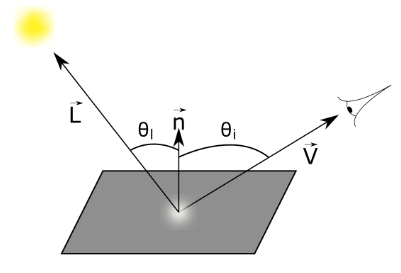
\includegraphics[scale=0.4]{reflec.png}
\caption{Superfície de incidência da luz.}
\label{fig:superficie}
\end{figure}


Para formalizar esse conceito uma superfície lambertiana plana, com o observador e fonte de luz na mesma posição é considerado. Desta forma, a intensidade da luz é constante para esse ângulos de iluminação constante. Desta forma, o ângulo incidente e de emissão são os mesmos. 

Num ponto (p,q) em análise no espaço gradiente, a normal à superfície é (p,1,-1). A seguinte equação é definida:

\begin{equation} 
R = r_{0}cos(\theta)
\label{eq:reflectancia}
\end{equation}

Em que R é a radiância, $\theta$ o ângulo de incidência da luz na superfície e r a constante de proporcionalidade da luz.

Então, definindo-se dois vetores unitários $n_{s}$ (na direção da fonte) e n (na direção normal a superfície), temos:

\begin{equation} 
n = \frac{(p,q,1)}{\sqrt{1+p^2+q^2}}
\end{equation}

Dado que $cos(\theta)=n.n_{s}$, então:

\begin{equation} 
R(q,p) = \frac{r_{0})}{\sqrt{1+p^2+q^2}}
\end{equation}

Portanto, $cos(\theta)$ corresponde, justamente, o brilho na imagem e o seu gráfico forma o espaço gradiente.

\chapter{Descrição da Proposta}\label{Descricao}

Esta seção é reservada para descrição de como é estruturada a sua solução, explicando em detalhes como as arquiteturas físicas e lógicas de suas soluções. 

Por exemplo, suponha um sistema desenvolvido em uma plataforma $X$, esta conectado a outros elementos para entrada e saída de sinais. Além disso, internamente, dentro do sistema desenvolvido em $X$, foi criado um procedimento para manipulação dos dados de entrada, realizando aquisição desse dados e os transmitindo por uma saída depois de realizar a computação.

No contexto descrito acima, as conexões que ligam $X$ aos demais dispositivos, os sinais, taxas de transmissão e número de bits para cada sinal (se for o caso) fazem parte da arquitetura física do sistema. Procure utilizar de imagens e/ou diagramas de blocos para descrever este elementos. Ex.: Figura \ref{fig:ArqLogSTRSD}.

\begin{figure}[ht]
    \centering
    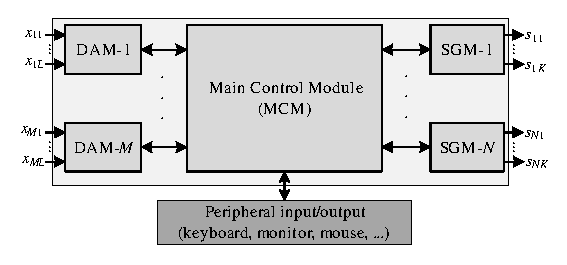
\includegraphics[width = 0.85\textwidth]{Imagens/Figura1.eps}
    \caption{Arquitetura Física em diagrama de bloco}
   	\label{fig:ArqLogSTRSD}
\end{figure}  

Já as funções que compõem os procedimentos internos do sistema devem ser descritas na arquitetura lógica. Nessa etapa, é importante descrever por meio de fluxogramas, Estados ou algum mecanismo que auxilie a ilustrar o fluxo de dados, ou seja, que mostre em detalhes o que acontece com os dados logo após a aquisição até chegar a saída (transmissão para algum outro dispositivo ou visualização).  Ex.: Figura \ref{fig:ATCT}.

\begin{figure}[ht]
\begin{center}
  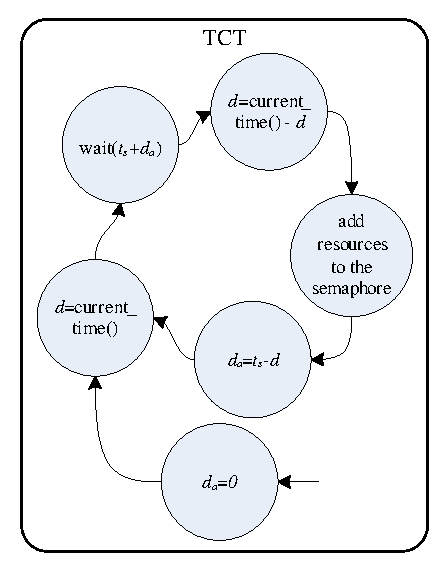
\includegraphics[width=7cm,height=9.13cm]{Imagens/Figura6.eps}\\
  \caption{Lógica para controle de tempo em um sistema baseado em Threads.}\label{fig:ATCT}
\end{center}
\end{figure}

É relevantes que tudo que seja descrito nesta seção seja genérico, ou seja, não tenha uma correlação explicita com o que foi desenvolvido. Isto melhora o aspecto organizacional do trabalho. Sendo assim, dados como valores numéricos, bem como os valores de cada parâmetro não precisam ser descritos nesta seção. Deixe isto para a seção de desenvolvimento e resultados.

\chapter{Desenvolvimento e Resultados}
   Nesta seção, se deve correlacionar o que foi descrito nas seções de \ref{Teoria} e \ref{Descricao}. Deve ser exposto o protótipo, os parâmetros utilizados, protocolos de comunicação, máquinas e plataformas para a prototipagem.
   
   É preciso descrever a metodologia de testes, como que tudo será testado.
   
   Ex.:
   Suponha a execução de um algoritmo com 3 parâmetros, Número de entradas, Número máximo de ciclos de execução e erro mínimo aceitável.
   \begin{itemize}
       \item Teste 1: Executar o precedimentos com os parâmetros: 1, 8, $10^{-1}$.
       \item Teste 2: Executar o precedimentos com os parâmetros: 10, 16, $10^{-2}$.
       \item Teste 3: Executar o precedimentos com os parâmetros: 50, 32, $10^{-4}$.
       \item Teste 4: Executar o precedimentos com os parâmetros: 100, 64, $10^{-5}$.
   \end{itemize}
   Deve-se também descrever como analisar o erro dos dados:
   
   Para analisar a confiabilidade dos resultados obtidos foram utilizadas medidas de erro entre os dados obtidos. As análises se baseiam no erro médio, erro quadrático médio e variância do erro.

    O cálculo do erro médio é demonstrado abaixo:

    \begin{equation}
    E_{m}(X) = \frac{1}{N}  \sum_{i=0}^{N-1}(X(i)-Y(i))
    \end{equation}
    em que, $E_m(X)$ é o valor do erro médio, $X(i)$ é o valor da i-ésima amostra coletada e $Y(i)$ é o valor da simulação em software nesse mesmo momento.

    O cálculo do erro médio quadrático é definido por 
    \begin{equation}
    E_{qm}(X) = \frac{1}{N}  \sum_{i=0}^{N-1}(X(i)-Y(i))^{2}
    \end{equation}
    em que, $E_qm(X)$ é o valor do erro médio quadrático, $X(i)$ é o valor da i-ésima amostra coletada e $Y(i)$ é o valor da simulação em software nesse mesmo momento.

    Para a variância, variável estatística que visa demonstrar o quanto que as amostras variam entorno de seu valor médio temos a seguinte equação
    \begin{equation}
    \sigma^{2}(E_{mq}) = \frac{1}{N}  \sum_{i=0}^{N-1}(E_{mq}(i)-\bar{E_{mq}})^{2}
    \end{equation}
    em que, $\sigma^2(E_{mq})$ é a variância da variável erro médio quadrático , $E_{mq}(i)$ é o i-ésimo valor do conjunto de amostras e $\bar{E_{mq}}$ é a média da variável em questão.
    
    Os resultados podem ser descritos das mais diversas formas. Procure utilizar todos os meios de descrição e ilustração para passar com mais clareza que o seu projeto atingiu os resultados esperados. 
    
    Sempre que inserir uma Tabela ou uma Figura, a descreva, não a deixe sem descrição, muito menos sem uma legenda clara.

\chapter{Conclusão}
    Breve conclusão referente ao trabalho realizado, se este atendeu as expectativas abordadas nos objetivos iniciais. 
    
%\bibliographystyle{abnt-alf}
\bibliography{referencias}
    Procure citar todas as referências utilizadas no projeto.

\end{document}